\documentclass{article}
\usepackage[utf8]{inputenc}
\usepackage{float}

\title{Distributed computing assignment 1: SOA}
\author{Zhong-Xi Lu, Angela Mizero, Thomas Van Bogaert}
\date{}

\usepackage{natbib}
\usepackage{graphicx}

\begin{document}

\maketitle

\section{Service Oriented Architecture}

\begin{figure}[H]
    \centering
    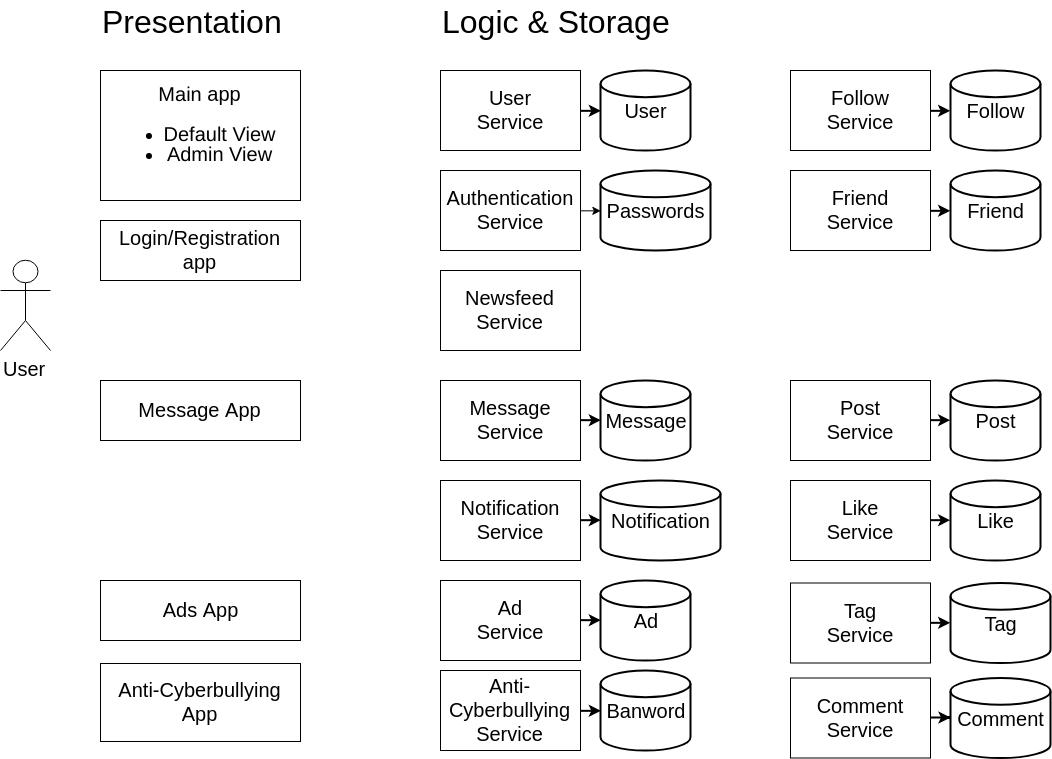
\includegraphics[width=\textwidth]{DC.png}
    \caption{Service oriented architecture}
    \label{soa}
\end{figure}

Our service oriented architecture consists of three layers, namely the presentation, logic and storage layer. In the front end we have different applications that each make use of our services. The main app also has two different views depending on their privilege (normal user or admin).

In the logic and storage layer, we have several microservices that all have their own API which will allow them to easily communicate with the outside. Most of these services also have their own database to store the necessary information. 

\section{API Services}

This section will go more into these microservices by precisely defining their REST API and their dependencies (what services they communicate with).

\begin{description}
    \item [User service:]
    \begin{description}
        \item[]
        \item[Dependencies:] Authentication service
    \end{description}
    \begin{description}
        \item[]
        \item[In:] POST users (email, username, password)
        \item[Out:] /
        \item[Logic:] Registers or creates a user
        \item[]
    \end{description}
    \begin{description}
        \item[In:] POST users/login (username, password)
        \item[Out:] Response indicating whether the login was successful or not (and return some token if it was successful)
        \item[Logic:] Tries to login a user
        \item[]
    \end{description}
    \begin{description}
        \item[In:] POST users/logout (token)
        \item[Out:] /
        \item[Logic:] Logs out a user
        \item[]
    \end{description}
    \begin{description}
        \item[In:] GET users
        \item[Out:] users (user\_id, email, username)
        \item[Logic:] Gets all the users
        \item[]
    \end{description}
    \begin{description}
        \item[In:] GET users/user/username
        \item[Out:] users (user\_id, email, username)
        \item[Logic:] Gets a user by username
        \item[]
    \end{description}
    \begin{description}
        \item[In:] GET users/user\_id
        \item[Out:] user (user\_id, email, username)
        \item[Logic:] Get a particular user
        \item[]
    \end{description}
    \begin{description}
        \item[In:] DELETE users/user\_id
        \item[Out:] /
        \item[Logic:] Deletes a user
        \item[]
    \end{description}
    \begin{description}
        \item[In:] PUT users/user\_id/block
        \item[Out:] /
        \item[Logic:] Blocks a user
        \item[]
    \end{description}
    \begin{description}
        \item[In:] PUT users/user\_id/unblock
        \item[Out:] /
        \item[Logic:] Unblocks a user
    \end{description}
\end{description}

\begin{description}
    \item [Authentication service:]
    \begin{description}
        \item[]
        \item[Dependencies:] /
    \end{description}
    \begin{description}
        \item[]
        \item[In:] POST password (user\_id, password)
        \item[Out:] /
        \item[Logic:] Adds user and password pair to the database to verify tokens in the future
    \end{description}
    \begin{description}
        \item[]
        \item[In:] DELETE password (user\_id)
        \item[Out:] /
        \item[Logic:] Remove password from the database
    \end{description}
    \begin{description}
        \item[]
        \item[In:] POST user (token)
        \item[Out:] Flag indicating whether the authentication was successful
        \item[Logic:] Tries to authenticate a user by checking the credentials
    \end{description}
\end{description}

\begin{description}
    \item [Message service:]
    \begin{description}
        \item[]
        \item[Dependencies:] Friend, notification service
    \end{description}
    \begin{description}
        \item[]
        \item[In:] POST message (contents, sender id, receiver id)
        \item[Out:] /
        \item[Logic:] Add message to DB
        \item[]
        
        \item[In:] GET messages/receiver\_id/sender\_id
        \item[Out:] All messages in conversation between receiver and sender (message: content, timestamp, id)
        \item[Logic:] Mark messages as read by receiver
    \end{description}
\end{description}

\begin{description}
    \item [Notification service:]
    \begin{description}
        \item[]
        \item[Dependencies:] /
    \end{description}
    \begin{description}
        \item[]
        \item[In:] POST notifications (notification contents, notification recipient(s) (UID))
        \item[Out:] /
        \item[Logic:] Add notification to DB
        \item[]
        
        \item[In:] GET notifications/user\_id 
        \item[Out:] Notifications (ID, timestamp, content)
        \item[Logic:] Mark notification as requested
        \item[]
        
        \item[In:] PUT notifications/notification\_id/user\_id
        \item[Out:] /
        \item[Logic: ] Mark notification as read
    \end{description}
\end{description}

\begin{description}
    \item [Ad service:]
    \begin{description}
        \item[]
        \item[Dependencies:] /
    \end{description}
    \begin{description}
        \item[]
        \item[In:] POST ads (contents, targeted users classes(s)) (user class example: "male" or "female")
        \item[Out:] /
        \item[Logic:] Add advertisement to DB
        \item[]
        
        \item[In:] GET ads/user\_id
        \item[Out:] Advertisement (contents)
        \item[Logic:] Increment view count of advertisement
        \item[]
        
		\item[In:] GET ads (may be used for administrator view)
        \item[Out:] List of all advertisements (target user class(es), contents)
    \end{description}
\end{description}

\begin{description}
    \item [Anti-Cyberbullying service:]
    \begin{description}
        \item[]
        \item[Dependencies:] /
    \end{description}
    \begin{description}
        \item[]
        \item[In:] POST anti\_cyberbullying (words seperated with a space)
        \item[Out:] /
        \item[Logic:] Words from wordlist get merged with existing words in DB
        \item[]

        \item[In:] GET anti\_cyberbullying
        \item[Out:] /
        \item[Logic:] Homepage for the anti\_cyberbullying service
        \item[]

        \item[In:] GET anti\_cyberbullying/bad\_words
        \item[Out:] All the bad words
        \item[Logic:] Get all the bad words from the database
        \item[]

        \item[In:] POST anti\_cyberbullying/contains\_bad\_word (sentence)
        \item[Out:] True if the provided sentence contains one or more bad words, false otherwise
        \item[Logic:] Check if there's a bad word in the sentence
    \end{description}
\end{description}

\begin{description}
    \item [Follow service:]
    \begin{description}
        \item[]
        \item[Dependencies:] /
    \end{description}
    \begin{description}
        \item[]
        \item[In:] POST follows (user\_id, other\_user\_id)
        \item[Out:] /
        \item[Logic:] User follows another user
        \item[]
    \end{description}
    \begin{description}
        \item[In:] DELETE follows/follow\_id
        \item[Out:] /
        \item[Logic:] Unfollow a user
        \item[]
    \end{description}
    \begin{description}
        \item[In:] GET follows/user/user\_id
        \item[Out:] Follows (follow\_id, user\_id, other\_user\_id)
        \item[Logic:] Get the list of people whom this user is following
        \item[]
    \end{description}
        \begin{description}
        \item[In:] GET followers/user/user\_id
        \item[Out:] Follows (follow\_id, user\_id, other\_user\_id)
        \item[Logic:] Get the list of people who are following this user
        \item[]
    \end{description}
    \begin{description}
        \item[In:] GET follows
        \item[Out:] Follows (follow\_id, user\_id, other\_user\_id)
        \item[Logic:] Gets all the follows
    \end{description}
\end{description}

\begin{description}
    \item [Friend service:]
    \begin{description}
        \item[]
        \item[Dependencies:] /
    \end{description}
    \begin{description}
        \item[]
        \item[In:] POST friends (user\_id, other\_user\_id)
        \item[Out:] /
        \item[Logic:] User is a friend of another user
        \item[]
    \end{description}
    \begin{description}
        \item[In:] DELETE friends/friend\_id
        \item[Out:] /
        \item[Logic:] Unfriend a user
        \item[]
    \end{description}
    \begin{description}
        \item[In:] GET friends/user\_id
        \item[Out:] Friends (friend\_id, user\_id, other\_user\_id)
        \item[Logic:] Gets the friends of a user
        \item[]
    \end{description}
    \begin{description}
        \item[In:] GET friends
        \item[Out:] Friends (friend\_id, user\_id, other\_user\_id)
        \item[Logic:] Gets all the friends
    \end{description}
\end{description}

\begin{description}
    \item [Newsfeed service:]
    \begin{description}
        \item[]
        \item[Dependencies:] Follow, Post service
    \end{description}
    \begin{description}
        \item[]
        \item[In:] GET newsfeed/user\_id
        \item[Out:] Posts
        \item[Logic:] Get the newsfeed of a user
    \end{description}
\end{description}

\begin{description}
    \item [Post service:]
    \begin{description}
        \item[]
        \item[Dependencies:] Follow, Notification, Tag service
    \end{description}
    \begin{description}
        \item[]
        \item[In:] POST posts (creator, content, tags)
        \item[Out:] /
        \item[Logic:] Create a new post
        \item[]

        \item[In:] GET posts/user/user\_id
        \item[Out:] Posts (post\_id, creator, timestamp, content)
        \item[Logic:] Get all the posts from a user
        \item[]

        \item[In:] GET posts/post\_id
        \item[Out:] Post (post\_id, creator, timestamp, content)
        \item[Logic:] Get a specific post
        \item[]

        \item[In:] DELETE posts/post\_id
        \item[Out:] /
        \item[Logic:] Delete a specific post
    \end{description}
\end{description}

\begin{description}
    \item [Like service:]
    \begin{description}
        \item[]
        \item[Dependencies:] /
    \end{description}
    \begin{description}
        \item[]
        \item[In:] POST likes (post\_id, user\_id)
        \item[Out:] /
        \item[Logic:] User likes a specific post
        \item[]

        \item[In:] GET likes/posts/post\_id
        \item[Out:] Likes (post\_id, user\_id)
        \item[Logic:] Get all the likes of a post
        \item[]

        \item[In:] DELETE likes/posts/post\_id (user\_id)
        \item[Out:] /
        \item[Logic:] Undo a like
        \item[]
    \end{description}
\end{description}

\begin{description}
    \item [Tag service:]
    \begin{description}
        \item[]
        \item[Dependencies:] /
    \end{description}
    \begin{description}
        \item[]
        \item[In:] POST tags (post\_id, user\_id's)
        \item[Out:] /
        \item[Logic:] Create user tags on a specific post
        \item[]

        \item[In:] GET tags/posts/post\_id
        \item[Out:] Tags (post\_id, user\_id)
        \item[Logic:] Get all the tags on a post
        \item[]
    \end{description}
\end{description}

\begin{description}
    \item [Comment service:]
    \begin{description}
        \item[]
        \item[Dependencies:] /
    \end{description}
    \begin{description}
        \item[]
        \item[In:] POST comments (post\_id, creator, content)
        \item[Out:] /
        \item[Logic:] Create a comment on a specific post
        \item[]

        \item[In:] GET comments/comment\_id
        \item[Out:] Comment (comment\_id, creator, timestamp, content)
        \item[Logic:] Get a specific comment
        \item[]

        \item[In:] GET comments/posts/post\_id
        \item[Out:] Comments (comment\_id, creator, timestamp, content)
        \item[Logic:] Get all the comments on a post
        \item[]

        \item[In:] DELETE comments/comment\_id
        \item[Out:] /
        \item[Logic:] Delete a comment
        \item[]
    \end{description}
\end{description}

\end{document}
